%%%%%%%%%%%%%%%%%%%%%%%%%%%%%%%%%%%%%%%%%%%%%%%%%%%%%%%%%%%%%%%%%%%%%%%%%%%%%%%
%
% Machine Learning
% 
%%%%%%%%%%%%%%%%%%%%%%%%%%%%%%%%%%%%%%%%%%%%%%%%%%%%%%%%%%%%%%%%%%%%%%%%%%%%%%%
\chapter{Machine Learning}
\label{cha4}

The field of Machine Learning contains concepts how computers can obtain information without explicitly programming this kind of information retrieval. These concepts of ''Learning'' can be divided into three main categories: Supervised learning, Unsupervised learning and Reinforcement Learning.

Supervised learning always deals with a user that ''feeds'' input to the program as well as desired output. The program should recognize patterns that lead from the given input parameters to the desired output.
Unsupervised learning instead, is an approach where the program does have an input and needs to find a structure in those data. The finding of some pattern can be the goal of the program itself.

Using reinforcement learning, every output of the program is being evaluated by the user again. The output that has been found correctly will be strengthened, whereas incorrect values will act repulsive on the algorithm. After multiple iterations of this process, the program can find the best answer (but not always the correct answer) using the attracting and repulsive values.

Our goal is to use one machine learning technique in order to improve the outcome of our application. One major objective that can be addressed with Machine Learning is the relation between accounting record positions and how they are assigned to all the accounts that are important for this position.
We identify two major problems regarding this classification:
\begin{enumerate}
         \item What does a position represent?
         \item Which accounts should be assigned to this position?
\end{enumerate}
As we are processing an invoice, we will retrieve a position as a String. An accountant would be able to identify the position (which means a semantic identification of the object) and assign it to the accounts that are important in this matter. But, as there is no concrete rule which position belongs to which accounts, every company can apply this position to different accounts.

For instance, the maintenance of a car in the carpool of a company could be booked as car costs, or (if the company defines it more specifically) as maintenance costs, car parts and worker time.
Hence we need an algorithm that is capable of the following:
\begin{enumerate}
		\item Assign involved accounts depending on the user (allow different account structure)
		\item Learn relationships between a string and a set of accounts
\end{enumerate}
While the algorithm should be able to deal with those problems, we will have another problem to deal with: OCR errors (e.g. ''CAB'' instead of ''CAR'')\footnote{We used uppercase letters here to make the possibility of OCR errors between those two words more easily understandable.} and similar words (e.g. plural words such as ''apples'' instead of ''apple''). 

Keeping those constraints in mind, we can start thinking about a Machine Learning technique that satisfies our goal or at least helps us to reach it.

\section{An abstract approach on accounting records}
\label{sec4.1}

Before we can compare different Machine Learning algorithms we have to think about the model that is used. On one hand, there is the position value which can be seen as a single String. On the other hand, we have 1195 Accounts (as proposed in the SKR03 account system\cite{datev12}\footnote{SKR03 and SKR04 are two branch-independent account systems proposed by DATEV eG. We only concentrate on one account system since the support of multiple account systems is not relevant for this thesis (see also section \ref{sec6.2})}.) that can be involved in this accounting process. Between those accounts, we also have to divide between accounts for debit and credit.

Evaluating each account per position would need two iterations: In a first iteration, the algorithm would need to determine whether the account is relevant for the string. The second iteration then would clarify the question about a credit or debit account.
We come up with a different approach. As we see the position abstract as a string, we see the combination of accounts as a combined structure. This way we do not only reduce the iterations to one but also enable a 1:1 relation.

For instance, given two accounts a$_1$ and a$_2$ we would have two possible structures: s$_1$: \{a$_1$$|$a$_2$\} and s$_2$: \{a$_2$$|$a$_1$\}\footnote{Each structure will be written the following way: The curly braces mark beginning and end of the structure, the pipe divides between credit and debit accounts.}. One time a$_1$ is related to the credit side, one time to the debit side and vice-versa for a$_2$. Given a position p$_1$, there are now two possible structures we can assign p$_1$ to.

The downside of this mapping from 1:N to 1:1 relations is the increasing number of possible solutions. But the advantage of it is the flexibility to assign a position to a known structure again after the user has defined how they want to it to be accounted.

\section{Possible machine learning algorithms}
\label{sec4.2}
We also need an accountant initially to define how the position should be accounted. After this information have been given, the algorithm is able to assign a similar position to the same structure of debit and credit accounts. This means that we will look for an algorithm in the field of supervised learning.

There are several well-known algorithms in this field. For instance, Artificial Neural Networks (ANN), the k-Nearest-Neighbour Algorithm (kNN) or Decision Trees. To select the appropriate algorithm for our problem, we will be using a randomly generated training set consisting of a combination of 30 positions and 9 different structures in 1920 cases. We will evaluate the performance and accuracy of some of these algorithms to find the one that suits the most by using a test set of 2000 positions to be tested. To do so, we will be using an open-source software (RapidMiner Studio) that enables us to switch between those algorithms and evaluate the accuracy before implementing them.

The following table shows the algorithms and the accuracy as well as the time needed to evaluate the result:

\begin{table}[!htb]
\centering
\scalebox{0.7}{
\begin{tabular}{@{}lcc@{}}
\toprule
Algorithm & \textbf{Accuracy} & \textbf{Duration} \\ \midrule
K-Nearest-Neighbour & 75,35\% & \textless1s \\ \midrule
Artifical Neural Network & 73,61\% & 30s \\ \midrule
Decision Trees & 72,92\% & \textless1s \\ \midrule
Na{\"i}ve Bayes & 72,92\% & \textless1s \\ \midrule
Random Forest & 55,03\% & \textless1s \\ \bottomrule
\end{tabular}%
}
\caption{Accuracy of different Machine Learning algorithms}
\label{mlAccuracy}
\end{table}

Except for the Random Forest algorithm, there is not much of a difference between the algorithms. While Decision Trees and Na{\"i}ve Bayes result in the same accuracy, ANN are slightly more accurate. The disadvantage of this algorithm is its duration that increases exponentially by the amount of data. The data that we used resulted in a duration of around 30 seconds execution time. The k-Nearest Neighbor algorithm instead, while still as fast as the other algorithms, also results in a higher accuracy.

We will now introduce the remaining three algorithms and take a closer look at the results regarding the data set that we used. After that, we will decide which algorithm we want to use in our application.

\subsection{The k-Nearest-Neighbor algorithm}
\label{sec4.2.1}
The kNN algorithm tries to classify an object by using \emph{k} neighbors of the object. Each of the \emph{k} neighbors already has a class \emph{c$_i$} which enables the calculation of a likelihood value for the unclassified object.
If we would choose \emph{k} = 1 then the object would be given the same class then the closest neighbor. But this can lead to wrong assumptions, since the only neighbor has been taken into account. Hence we would need to select a value for \emph{k} $>$ 1. The given accuracy from Table \ref{mlAccuracy} has been achieved with \emph{k} = 5.

The neighbor calculation works the following way: For \emph{n} attributes, calculate the euclidean distance between the given attribute value for the object to be classified (\emph{x}) and \emph{y}:
\[
d(x, y) = \sum\limits_{i=1}^n \sqrt{x_i^2 - y_i^1}
\]
Take the \emph{k} examples closest to \emph{x} and label \emph{x} with the class distributed the most amongst these neighbors.

When further investigating in the results provided by the algorithm we found something we did not expect. In our training data, we defined a position p$_1$ and two different structures s$_1$ and s$_2$. \emph{n} times p$_1$ has been classified to s$_1$, and \emph{n} times to s$_2$. This means p$_1$ is equally distributed between those two classes. But the kNN algorithm resulted in a classification of s$_1$ = 60\% and s$_2$ = 40\%. This can be explained by the chosen value for \emph{k}. As we defined \emph{k} = 5, there were 5 neighbors, $\frac{2}{5}$ that belonged to s$_2$ and $\frac{3}{5}$ that belonged to s$_1$. And indeed, as we changed \emph{k} to an even value (\emph{k} = 6) we had the expected classification of 50\% for s$_1$ and 50\% for s$_2$.

This should be taken into consideration when using this algorithm. As we do not know how much different classes exist and the amount of classes can increase by the user assigning positions to new structures, we could have wrong classification values.

\subsection{Decision Trees}
\label{sec4.2.2}
Decision Trees are a simple and still effective way of classifying an object to different classes. Usually, the object that should be classified contains several attributes and each of them will be taken into consideration iteratively.

We want to explain the behavior of decision trees on the following example: 
A telecommunication company had an increasing amount of customer loss recently. To find out the reasons behind that and to find out which actions to take to get new customers again, they build up a tree with the data they have of their customers. This decision tree can be seen in figure \ref{decisionTreeExample}.

\begin{figure}[ht!]
\centering
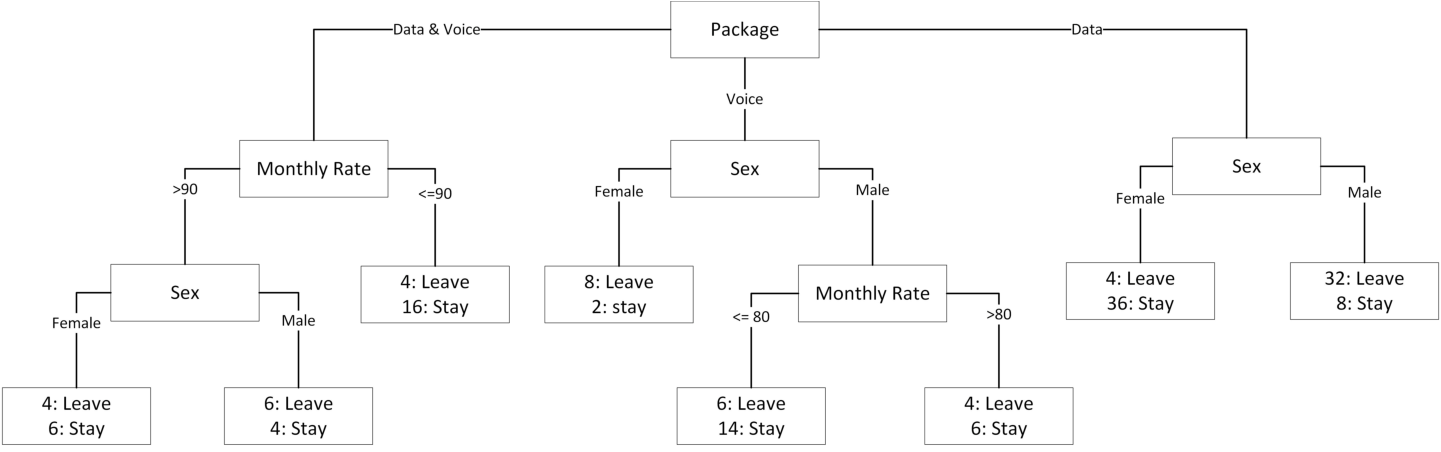
\includegraphics[width=\textwidth,natwidth=244,natheight=76]{Images/ML/DecisionTreeExample.pdf}
\caption{Example of a decision tree \label{decisionTreeExample}}
\end{figure}

The companies offer three packages to their customers: Data, Voice and Data \& Voice. The data package has a high amount of male customers that left, whereas the most of the female customers stayed with the companies offer. The Voice package shows a difference between male customers that have been charged over 80 monetary units and the customers with a maximum of 80 monetary units.

Hence it is very likely that reducing the monthly rate for this package will result in a higher amount of customers staying with the offer of the company.

Using this decision tree, it is possible to split between objects even further, using different attributes. In our case, we only have the position as an attribute. If we would apply a decision tree to this problem, it would result in a tree with a depth of 1. This way the actual idea behind the decision tree is not used. The results would still be valid, though.

\subsection{Na{\"i}ve Bayes}
\label{sec4.2.3}
Na{\"i}ve Bayes is a simple probabilistic classifier that calculates the probability that an object belongs to a class by taking each attribute of the object and comparing it with the probability of this attribute in the given class.

The probability that object \emph{x} belongs to the class \emph{c$_j$} can be calculated by the following way: For each of the \emph{n} attributes, get the probabilistic value that the attribute \emph{x$_i$} belongs to the class \emph{c$_j$}. The product sum of all those values will result in the probability for the class \emph{c$_j$}.
\[
P(x|c_j) = \prod\limits_{i=1}^n P(x_i|c_j)
\]
After that, the most likely class can be retrieved by simply taking the maximum of those probabilities.

What this means for our case is the following: As we do not have any additional information on the position, the only attribute there is is the string itself. This attribute is compared with the already classified positions. The result of this calculation will basically assign the position \emph{p} to the class that has the most positions that are similar to \emph{p}.

In addition to that, a way to improve the comparison is to use a numerical value that represents the similarity between the position \emph{}p and another position that \emph{p} is compared with. This can be done using the Levenshtein distance. The distance value represents the number of changes needed to transform one position to the other. Using a relative value, we can make this result relative by the size of the position string:

\[
\frac {\text{Levenshtein distance}}{\text{Length of the position}}
\]

\section{Decision finding and explanation}
\label{sec4.3}

While we have excluded Random Forests due to the low accuracy as well as Artificial Neural Networks because of the long execution time from our list of choices, there are still three possible Machine Learning algorithms under consideration. We will now explain advantages and disadvantages of these algorithms and conclude this chapter by selecting one of these algorithms for our application.

All of the three algorithms are relatively easy to implement, the underlying concept is easily understandable, compared with more sophisticated Machine Learning algorithms, and the resulting output of one of these algorithms is reasonable and traceable. 

As already mentioned in section \ref{sec4.2.2}, the concept of a decision tree would not be completely used in our given problem. Decision trees are based on objects with multiple attributes and this can not be provided by our problem. Hence we will not use Decision Trees in our application.

Another problem has been mentioned in section \ref{sec4.2.1} before. When using the kNN classifier, the size of \emph{k} has to be selected. Using a small \emph{k} can lead to the wrong classifications because of a bad classified neighbor. Choosing a high \emph{k} could also lead to overfitting and would reduce the effectiveness of our method. But, since the number of possible classes can (and will) increase over time, we would need to adjust \emph{k} every time and therefore use another algorithm. Hence the usage of the kNN algorithm will not be considered anymore.
This means, that we will use a Na{\"i}ve Bayes approach in our application to classify positions to structures. 